\chapter{InSAR技术原理}

\section{SAR与InSAR原理}

\subsection{SAR}

SAR由传统的雷达技术发展而来。
通过水平向和垂直向的压缩成像技术能够实现以较小的雷达天线
得到较高空间分辨率的影像。
每幅SAR影像的数据为光波从天线到地面每一个像素点然后反射再被天线接受的相位延迟。
即
\begin{equation}
    \phi=-\frac{4\pi}{\lambda}r
\end{equation}

\subsection{InSAR}

如果对于同一块区域有两幅影像,就可以对两幅影像做干涉处理。
原理如图\ref{fig:geometry}所示。
\begin{figure}[htb!]
    \centering
    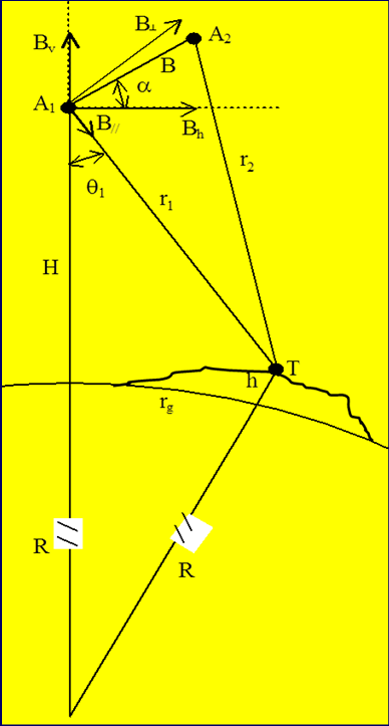
\includegraphics[width=0.5\textwidth]{geometry.png}
    \caption{InSAR技术原理示意图}
    \label{fig:geometry}
\end{figure}
所谓干涉,就是指二者相位相减。即
\begin{equation}
    \Delta \phi=-\frac{4\pi}{\lambda}(r_1-r_2)
\end{equation}
其中$\Delta r$为卫星视线方向的变化。
注意这里讨论的只是忽略大气效应即其他失相干效应,只考虑理想情况。
通常情况下,两幅影像并不是在相同的位置拍摄,二者之间有一定的距离。
所以当不存在任何的地表形变的情况下,可以通过一些几何的参数将此变化表达出来。
\begin{equation}
    \Delta \phi=\frac{4\pi}{\lambda}\left(\sqrt{r_1^2−2(B_hsinθ_1−B_{\perp}sinθ_1)r_1+B^2}−r_1\right)
\end{equation}

如果已知数字高程模型的话,可以算出来在理想条件下,无形变时的相位差。
将实际算得的相位差和无形变时理论计算的相位差相减,剩余的相位差即为因形变引起的相位差。
\begin{equation}
    \Delta \phi_{r}=-\frac{4\pi}{\lambda}u_{LOS}
\end{equation}
其中,$u_{LOS}$为地表形变在卫星视线(line-of-site:LOS)方向的投影,
从而可以把地表在卫星视线方向的形变算出来。
这种技术称之为D-InSAR。

注意,实际的到的相位是“缠绕”的相位,即相位是处于$(-\pi,\pi]$之间的。
将缠绕的相位通过解缠操作之后才得到上文中使用的相位。
解缠的方法很多,基本的假设是相邻像素的相位差不超过$\pi$。





